\documentclass[10pt,a4paper]{book}
\usepackage[utf8]{inputenc}
\usepackage{amsmath}
\usepackage{amsfonts}
\usepackage{amssymb}
\usepackage{graphicx}
\usepackage[left=2cm,right=2cm,top=2cm,bottom=2cm]{geometry}
\author{Stefan Kraatz, IMT\\Vorlesungsmitschrift}
\title{Entwicklung von Software Systemen}
\begin{document}
\maketitle
\chapter{eins}
\chapter{zwei}
\section{}
\section{}
\section{Zahlendarstellungen}
(VL 30.10.2012) Was ist die Semantik (Bedeutung) von Wertliteralen \ (G\_Wertliterale, R\_Wertliterale\ ) für Zahlen?
\chapter{Systemanalyse/Produktdefinition}
\section{}
(VL 02.11.2012) (Bild : Modellierungsperspektiven) 
\section{Modellierung von Systemfunktionen}
\subsection{Geschäftsprozessmodelle}
\subsection{Datenflussdiagramme (DFD)}
(VL 06.12.2012)
Notizen: Bestand der Structured Analysis (SA) and System Specification $\rightarrow$ Tom de Marco (1987); auch "data flow diagram"
\\
\\
Ein DFD beschreibt
\begin{itemize}
  \item Wege von Daten zwischen Verarbeitungsfunktionen, Speicher und Schnittstellen und die \underline{Transformation} der Daten durch die Funktionen.
  \item ein "laufendes System", d.h. Aspekte wie Initialisierung/Terminierung werden ignoriert.
  \item $\rightarrow$ \underline{keinen} sequenziellen Ablauf, sondern nur Daten- u. Funktionsabhängigkeiten.
\end{itemize}
\subsubsection*{Diagrammnotation}
\begin{itemize}
  \item Datenfluss (Bild: Datenfluss)
  \item Funktion/Prozess (Bild Funktion/Prozess)
  \item Datenspeicher (Bild: Datenspeicher)
  \item Schnittstelle (Bild: Schnittstelle)
\end{itemize}
$\Rightarrow$ Netze/Graphen aus
\begin{itemize}
  \item Funktionen, Datenspreichern und Schnittstellen als Knoten
  \item Datenflüssen als Kanten
\end{itemize}
\subsubsection*{Regeln zum Aufbau von DFD}
syntaktische Bedingungen:
\begin{itemize}
  \item mindestens eine Schnittstelle
  \item eindeutige Namen (jeder Schnittstellen-, Funktions-und Speichername existiert  \underline{nur einmal} in einem DFD) 
  \item Datenflüsse beginnen und enden immer in einer Funktion
  
   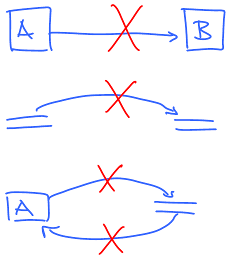
\includegraphics[scale=1,width=230pt,height=270pt]{EvSBook_Src/3_2_1__07.png}
  \item jeder Datenfluss (Kante im DFD) ist mit einem Datennamen (Datentyp) bezeichnet\\  \emph{Ausnahme:} DFD von oder zu einem Speicher der den gesamten Speicher transportiert (Datum des Typs des Speichers)
\end{itemize}
semantische Bedingungen:
\begin{itemize}
  \item DFD beschreibt keinen Kontrollfluss (keine Ansage der Reihenfolge der Verarbeitung durch Funktionen, Verzweigungen, Wiederholungen) 
  \item Schnittstellen repräsentieren (Typen von) Akteure(n), das heisst Personen in Rollen, Geräten, Verbindungen zu anderen Systemen 
  \item Funktionsnamen in Form von : (Verb + Objekt) oder (Objekt+Verb)
  \item Datenflussnamen in Form von : [Adjektiv] Substantiv (keine Verbformen) 
\end{itemize}
Funktionen, Speicher, Datenflüsse können \underline(verfeinert) (detailliert) werden; (zB Funktion wird durch Teilfunktion realisiert). 

$\rightarrow$ Zerlegung in Teilspeicher, Teilfunktionen, Teildatenflüsse

$\Rightarrow$ DFD werden i.A. als hierarchische Strukturen konstruiert.

Geht noch weiter \ldots
\section{Modellierung von Daten}
\subsection{Datenlexikon, Data Dictionary (DD)}
\end{document}